\documentclass[border=6pt]{standalone}
% Shared preamble for web figures.  Each figure is a standalone .tex that
% \input's this file; scripts/make-figures.sh turns it into an SVG.
% Handouts pull the same file with \fig{Unit_X/<name>}.
\usepackage[T1]{fontenc}
\usepackage{helvet}
\renewcommand{\familydefault}{\sfdefault}
\renewcommand{\ttdefault}{pcr}  % Courier: a real Type 1 typewriter font
\usepackage{amsmath}
\usepackage{tikz}
\usetikzlibrary{arrows.meta,positioning,calc,shapes.symbols,shapes.geometric}

% Who makes the rules is the point of most diagrams in this book, so the
% colors mean the same thing everywhere: blue is a person, orange is the
% computer, green is an answer, pink is the human brain.
\definecolor{person}{HTML}{2C6FAE}
\definecolor{machine}{HTML}{D35400}
\definecolor{result}{HTML}{1E8449}
\definecolor{brainpink}{HTML}{C2185B}
\definecolor{ink}{HTML}{2C3E50}

\tikzset{
  doodle/.style={line width=1.5pt, line cap=round, line join=round, draw=ink},
  box/.style={draw, rounded corners=5pt, line width=1.1pt, align=center,
              inner sep=7pt, minimum height=1.0cm, font=\small},
  personbox/.style={box, draw=person, fill=person!10},
  machinebox/.style={box, draw=machine, fill=machine!10},
  resultbox/.style={box, draw=result, fill=result!10},
  plainbox/.style={box, draw=ink!70, fill=ink!4},
  flow/.style={-{Stealth[length=8pt]}, line width=1.4pt, draw=ink},
}

% A person (blue) and a robot head (orange) as small icons.
% \personicon{x}{y}{scale}   \roboticon{x}{y}{scale}
\newcommand{\personicon}[3]{%
  \begin{scope}[shift={(#1,#2)}, scale=#3]
    \fill[person] (0,0.62) circle (0.28);
    \fill[person, rounded corners=6pt] (-0.42,-0.55) rectangle (0.42,0.28);
  \end{scope}}
\newcommand{\roboticon}[3]{%
  \begin{scope}[shift={(#1,#2)}, scale=#3]
    \draw[machine, line width=1.2pt] (0,0.5) -- (0,0.72);
    \fill[machine] (0,0.78) circle (0.08);
    \draw[machine, line width=1.4pt, fill=machine!12, rounded corners=4pt] (-0.5,-0.45) rectangle (0.5,0.5);
    \fill[ink] (-0.2,0.12) circle (0.08);
    \fill[ink] (0.2,0.12) circle (0.08);
    \draw[ink, line width=1pt] (-0.22,-0.22) -- (0.22,-0.22);
  \end{scope}}

\begin{document}
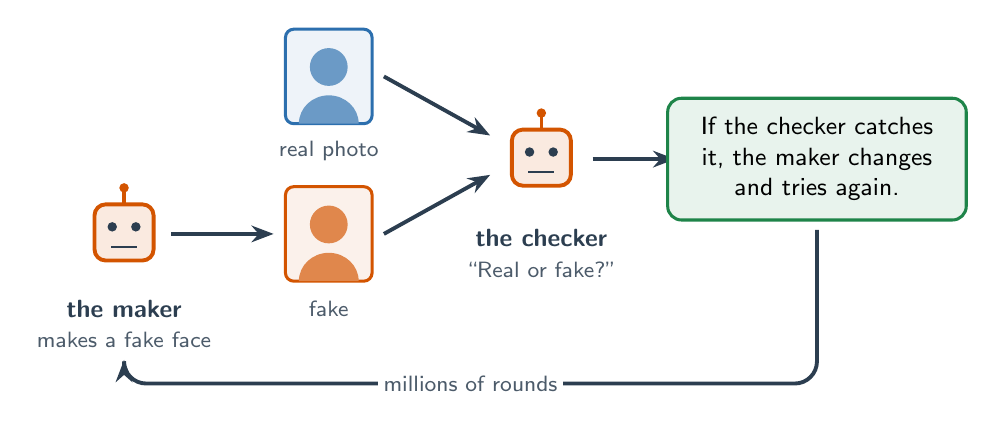
\begin{tikzpicture}[
  ttl/.style={font=\small\bfseries, text=ink, align=center},
  sub/.style={font=\footnotesize, text=ink!85, align=center},
]
% A GAN: a maker network and a checker network play a game.
\newcommand{\face}[3]{% x, y, color
  \begin{scope}[shift={(#1,#2)}]
    \draw[#3, line width=1.1pt, fill=#3!8, rounded corners=3pt] (-0.55,-0.6) rectangle (0.55,0.6);
    \fill[#3!70] (0,0.12) circle (0.24);
    \fill[#3!70] (-0.38,-0.6) arc (180:0:0.38 and 0.36) -- cycle;
  \end{scope}}
\roboticon{0}{0}{0.75}
\node[ttl] at (0,-0.95) {the maker};
\node[sub] at (0,-1.35) {makes a fake face};
\draw[flow] (0.6,0) -- (1.9,0);
\face{2.6}{0}{machine}
\node[sub] at (2.6,-0.95) {fake};
\face{2.6}{2.0}{person}
\node[sub] at (2.6,1.05) {real photo};
\draw[flow] (3.3,0) -- (4.65,0.75);
\draw[flow] (3.3,2.0) -- (4.65,1.25);
\roboticon{5.3}{0.95}{0.75}
\node[ttl] at (5.3,-0.05) {the checker};
\node[sub] at (5.3,-0.45) {``Real or fake?''};
\draw[flow] (5.95,0.95) -- (7.0,0.95);
\node[resultbox, font=\small, text width=3.3cm] at (8.8,0.95) {If the checker catches it, the maker changes and tries again.};
\draw[flow, rounded corners=8pt] (8.8,0.05) -- (8.8,-1.9) -- (0,-1.9) -- (0,-1.6);
\node[sub, fill=white, inner sep=2pt] at (4.4,-1.9) {millions of rounds};
\end{tikzpicture}
\end{document}
